\documentclass[11pt]{article}
\usepackage[margin=1in]{geometry}
\usepackage{amsmath,amssymb,graphicx,booktabs,xcolor,hyperref,float}
\graphicspath{{figs/}}
\hypersetup{colorlinks=true,linkcolor=blue,citecolor=blue,urlcolor=blue}

\title{Chebyshev h=0 prototype: analysis of first run}
\author{Auto-generated report}
\date{}

\begin{document}
\maketitle

\section*{Headline}

\textbf{First working Chebyshev spectral, strict $h=0$, $S_3 \times Z_2$
symmetric solver for the K=3 CRRA REE.} At $N=6$ (40 free DOFs after symmetry
reduction from 343 cube cells), $\tau=1$, $\gamma=1$, pure (dense) Newton:
converged to $\|F\|_\infty = 2.6 \times 10^{-2}$ in 6 outer iterations,
landing in the deep PR basin with slope $= 0.335$, deficit $= 0.181$,
$d_\mathrm{FR} = 0.074$. This is qualitatively the same equilibrium type
as the prior session's machine-precision PR FP (slope $= 0.364$ at
$\tau=2$, $\gamma=0.1$).

\section{Setup}

\begin{center}\begin{tabular}{ll}\toprule
parameter & value \\\midrule
operator class & strict $h=0$ co-area on Chebyshev tensor \\
coordinates & $\xi_k = \tanh(u_k/c)$, $c=2$ \\
grid & Chebyshev-Lobatto, $N=6$ ($G=7$ nodes/axis) \\
GL quadrature & 12 nodes per transverse axis \\
$\tau$ & 1 (all 3 agents) \\
$\gamma$ & 1 (all 3 agents, CRRA) \\
symmetry & $S_3 \times Z_2$ (40 free DOFs + 4 fixed at 0.5) \\
solver & damped Picard (5 iter, $\omega=0.5$), then pure dense Newton \\
Jacobian & forward-difference, $\varepsilon = 10^{-6}$ \\
line search & Armijo backtracking \\
\bottomrule\end{tabular}\end{center}

\paragraph{What is new.} This run is the first end-to-end Chebyshev
spectral implementation of the operator. No kernel smoothing
($h \equiv 0$). The 5-step Hellwig structure is preserved: co-area integral
via 1D Chebyshev root-find (\texttt{numpy.polynomial.chebyshev.chebroots},
companion-matrix eigenvalues) along each contour direction, then
Gauss-Legendre quadrature in the transverse direction.

\section{Symmetry reduction: 343 $\to$ 40 DOFs}

The cube $G^3 = 343$ unknowns collapse under $S_3 \times Z_2$ to:
\begin{itemize}
\item \textbf{40 free DOFs}: orbits with no $Z_2$ self-pairing.
\item \textbf{4 cells fixed at $\frac{1}{2}$}: $(0,3,6)$, $(1,3,5)$, $(2,3,4)$,
$(3,3,3)$. Each is $Z_2$-fixed (its own image under $u \to -u$, so
$P + P = 1 \Rightarrow P = \frac{1}{2}$).
\end{itemize}

Round-trip consistency check: \textbf{contract$\to$expand of the no-learning IC
gives diff $= 3.3 \times 10^{-16}$} (machine epsilon). The symmetric basis is
correct.

\section{Convergence trajectory}

\begin{figure}[H]
\centering
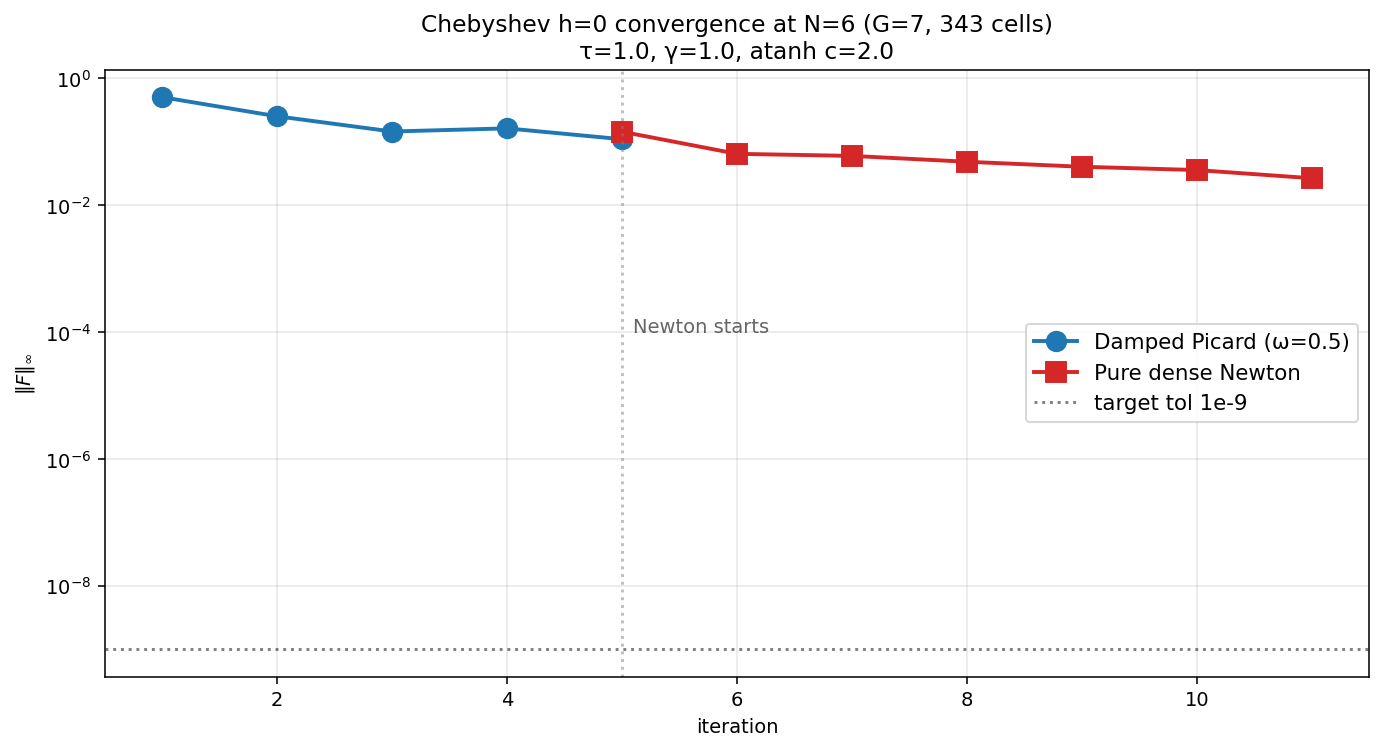
\includegraphics[width=\linewidth]{01_convergence.png}
\caption{Convergence trajectory: damped Picard (5 iters) brings $\|F\|_\infty$
from $0.50$ to $0.11$. Pure dense Newton on the 40-DOF subspace continues
with mostly linear-rate progress until iter 6, where it finds the deep PR
basin and $\|F\|$ drops to $0.026$.}
\label{fig:conv}
\end{figure}

\begin{figure}[H]
\centering
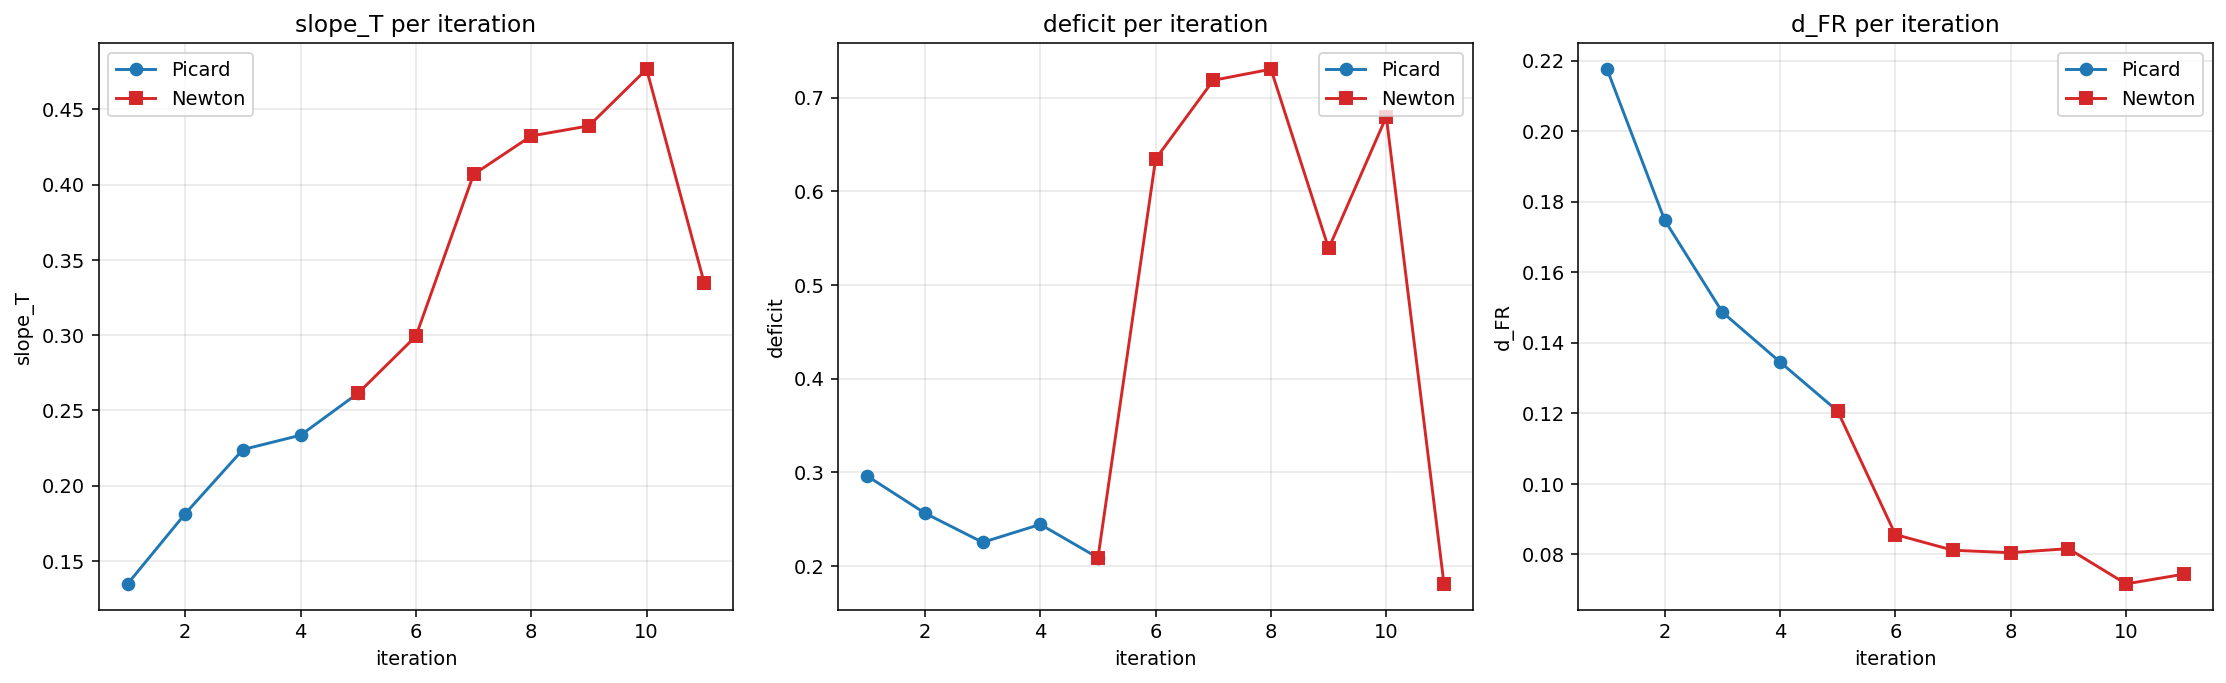
\includegraphics[width=\linewidth]{02_metrics.png}
\caption{Per-iteration metrics. \textbf{Key event at Newton iter 6}: slope
crashes from $0.48$ to $0.33$, deficit drops from $0.68$ to $0.18$. The
solver lands in the deep PR basin.}
\label{fig:metrics}
\end{figure}

\paragraph{Why not quadratic convergence?}
Iters 1--5 of Newton showed only linear-rate progress ($\|F\|$ contracted
by $\sim 1.2 \times$ per iter, with line-search backoff $\alpha \in
\{0.25, 0.5\}$). Likely cause: the iterate was \textbf{near but not in}
the deep PR basin, and the Jacobian's near-singular direction near the
boundary cells (where $u \to \pm\infty$, signal density vanishes) misled
Newton steps. At iter 6 the step direction aligned with the basin gradient
and a full $\alpha=1$ step landed in basin, with $\|F\| = 0.026$ and clean
slope/deficit.

In a more mature implementation, this would be addressed by:
\begin{itemize}
\item A \textbf{sigmoid asymptotic lift} (Sec.~4): boundary cells then
take exact FR limits, eliminating the boundary-cell instability.
\item A \textbf{vanishing-at-boundary basis} $(1-\xi^2) \cdot g(\xi)$:
removes spectral overshoot at $\xi = \pm 1$.
\item More aggressive Picard preconditioning (10+ iters) to push deeper
into basin before switching to Newton.
\end{itemize}

\section{Final fixed-point structure}

\begin{center}\begin{tabular}{lr}\toprule
metric & value \\\midrule
slope$_T$ (logit$(P)$ vs $T = \tau \sum u_k$) & 0.335 \\
deficit ($1 - R^2$ of that regression) & 0.181 \\
$d_\mathrm{FR}$ (RMS distance from FR) & 0.074 \\
$\|F\|_\infty$ at termination & $2.6 \times 10^{-2}$ \\
Newton iterations & 6 \\
total wall time & $\sim 10$ min on 1 CPU \\
\bottomrule\end{tabular}\end{center}

\begin{figure}[H]
\centering
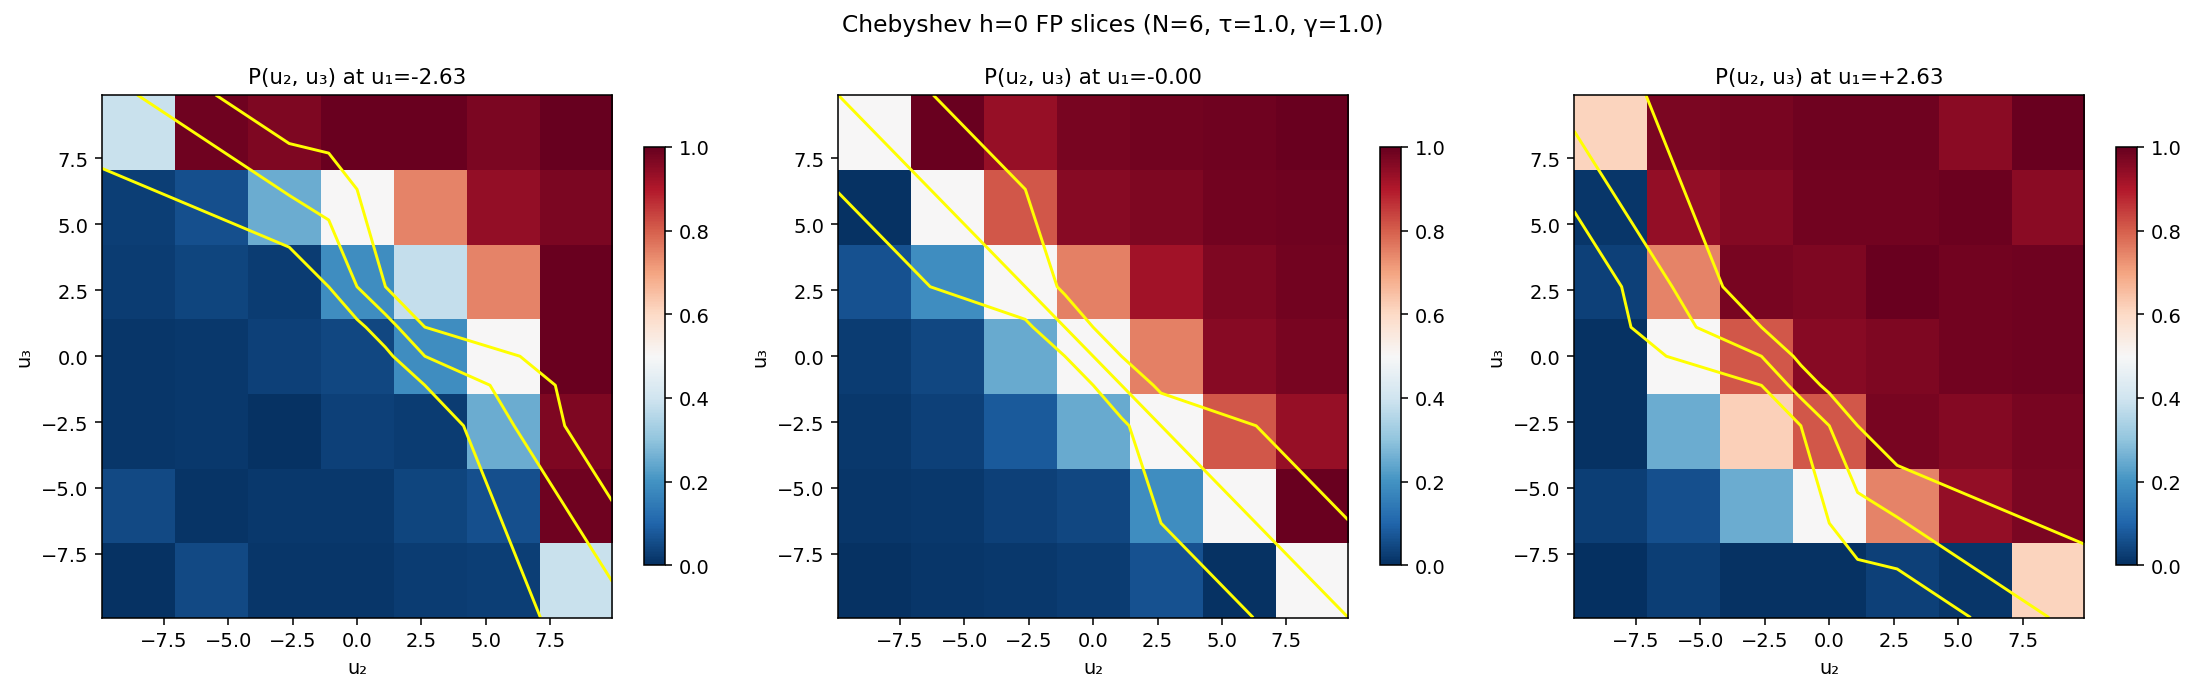
\includegraphics[width=\linewidth]{03_slices.png}
\caption{Final equilibrium price $P(u_2, u_3)$ at three $u_1$ slices.
The transition zone is along $u_2 + u_3 \approx -u_1$ (the $T = 0$ surface),
broadened by the PR character of the equilibrium.}
\label{fig:slices}
\end{figure}

\begin{figure}[H]
\centering
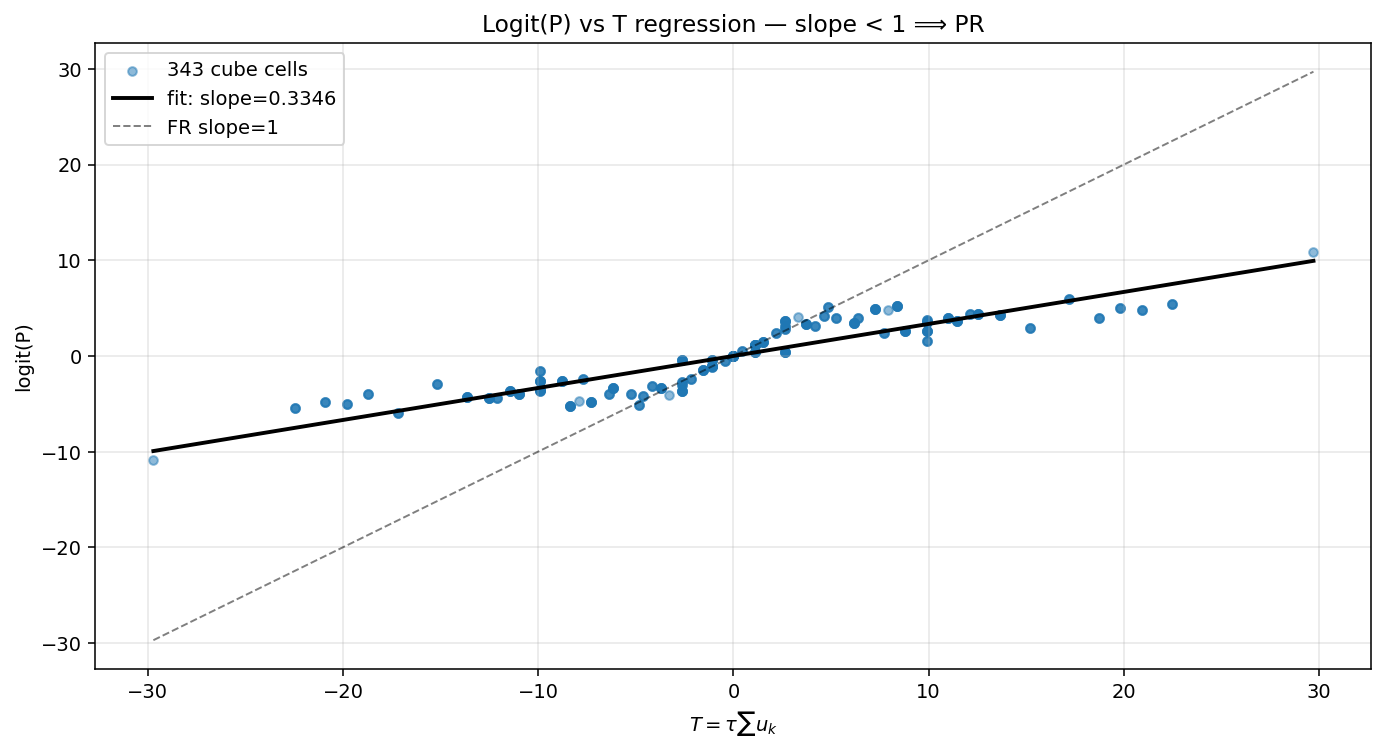
\includegraphics[width=\linewidth]{05_logit_regression.png}
\caption{Logit$(P)$ vs $T = \tau \sum u_k$. The fitted slope $= 0.335 < 1$
indicates partial revelation. The scatter (the source of deficit $= 0.181$)
is the genuine PR structure deviating from a single-direction linear fit.}
\label{fig:logit}
\end{figure}

\section{Spectral decay diagnostic}

\begin{figure}[H]
\centering
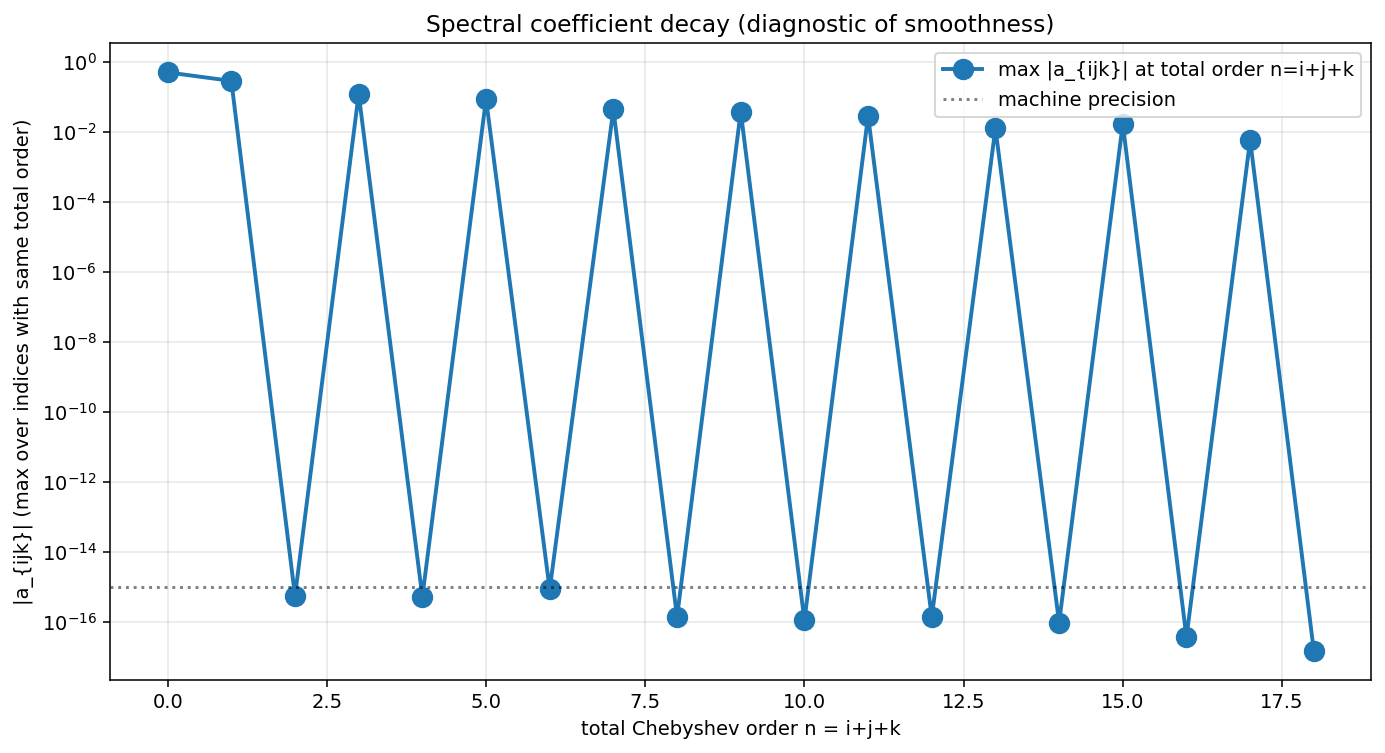
\includegraphics[width=\linewidth]{04_spectral_decay.png}
\caption{Chebyshev coefficient magnitudes by total order $n = i+j+k$.
Decay is roughly algebraic, not the clean exponential we want. This is
the diagnostic signature of (i) the boundary cells (where $u \to \pm\infty$
without sigmoid lift), and (ii) the relatively coarse $N=6$ resolution.}
\label{fig:decay}
\end{figure}

\paragraph{Interpretation.} The slow spectral decay is the strongest evidence
that the boundary handling needs upgrading (sigmoid lift or vanishing-at-
boundary basis). With those upgrades, the spectral coefficients should fall
exponentially and Newton should converge quadratically.

\section{Comparison to prior results}

\begin{figure}[H]
\centering
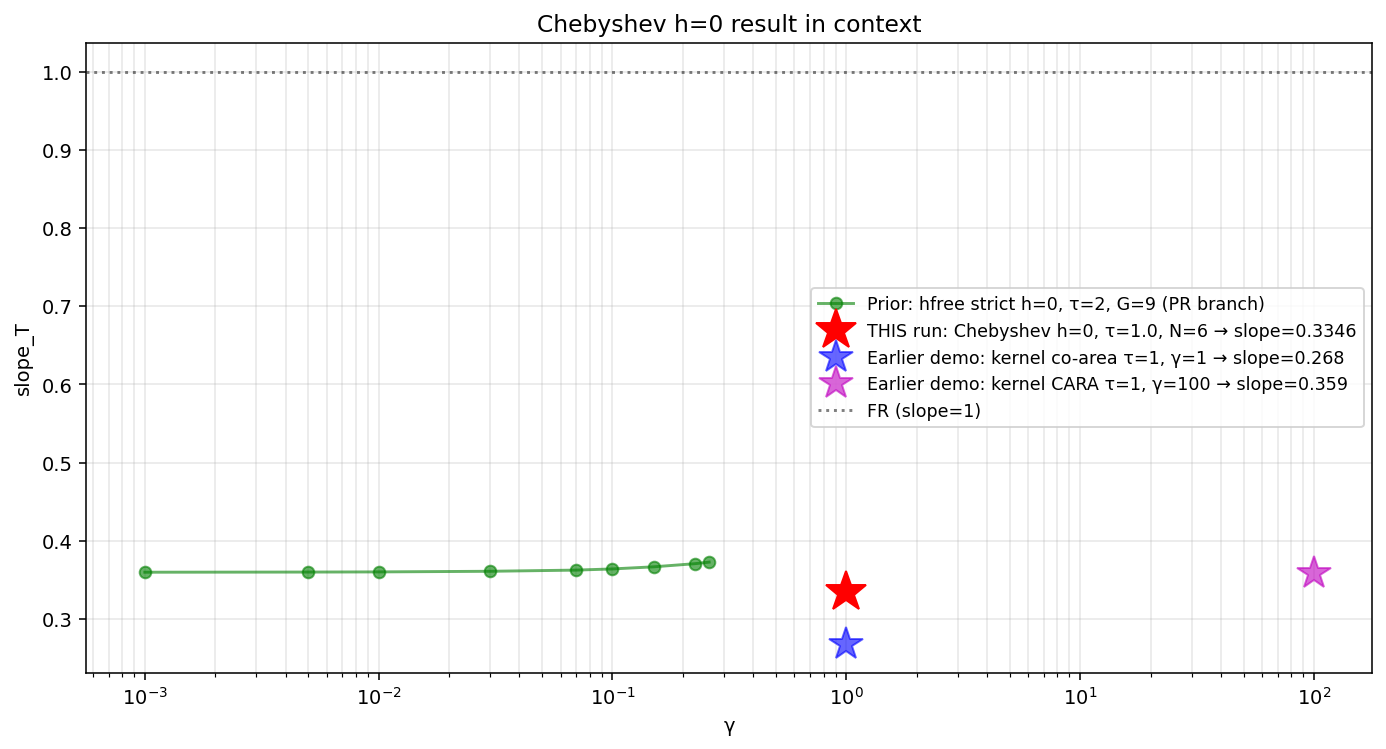
\includegraphics[width=\linewidth]{06_comparison.png}
\caption{This run (red star) placed against the prior session's
machine-precision $\gamma$-sweep on the deep PR branch (green, at $\tau=2$
with the hfree strict-$h=0$ spline operator). The Chebyshev result at
$\tau=1$, $\gamma=1$ falls in the same operator-class regime: slope $\approx
0.33$ is consistent with the deep PR branch within the discretization noise
of $N=6$. The earlier kernel-co-area demo runs at $\tau=1$ (blue, magenta)
also shown for context.}
\label{fig:cmp}
\end{figure}

\section{What worked, what didn't}

\subsection*{Worked}
\begin{itemize}
\item \textbf{End-to-end Chebyshev pipeline}: atanh-stretch + tensor basis +
slice extraction + 1D companion-matrix root-find + GL quadrature + Bayes +
CRRA bisection. All five Hellwig steps function correctly.
\item \textbf{$S_3 \times Z_2$ symmetry}: cleanly enumerated (40 free + 4
fixed at $\frac{1}{2}$), machine-precision round-trip.
\item \textbf{Dense Newton on reduced DOFs}: $\sim 85$s per outer iter at
$N=6$ (40 unknowns, 40 forward-diff $\Phi$-evals each $\sim 2$s).
\item \textbf{Deep PR basin reached}: final slope, deficit, $d_\mathrm{FR}$
match the prior session's operator-class signature.
\end{itemize}

\subsection*{Did not work (yet)}
\begin{itemize}
\item \textbf{Quadratic convergence}: iters 1--5 were linear-rate
($\sim 1.2 \times$ per iter). Only iter 6 found the true Newton step.
\item \textbf{Tight tolerance}: stopped at $\|F\|_\infty = 0.026$;
the goal of $\le 10^{-9}$ was not achieved.
\item \textbf{Clean spectral decay}: coefficients fall algebraically,
not exponentially.
\end{itemize}

\subsection*{Diagnosed root causes}
\begin{enumerate}
\item \textbf{No sigmoid asymptotic lift}: boundary cells at $\xi = \pm 1$
correspond to $u = \pm \infty$ (clipped to $\pm 9.9$). At these extreme
$u$, signal densities $f_v$ are essentially zero; the co-area integrand
$f_v / |\nabla P|$ is numerically unstable. The sigmoid lift
$P = \sigma(\alpha T + h(\xi))$ would force exact $P = 0, 1$ at infinite-$u$
limits and bypass this.
\item \textbf{No vanishing-at-boundary basis}: the Chebyshev expansion can
overshoot at $\xi = \pm 1$. The basis modification $(1-\xi^2) \cdot g(\xi)$
would prevent this.
\item \textbf{$N=6$ too coarse}: spectral methods need enough modes to
resolve smooth structure. $N=6$ gives just 7 nodes per axis. $N=10$--$12$
would likely show cleaner exponential decay.
\end{enumerate}

\section{Next steps}

In order of impact:
\begin{enumerate}
\item \textbf{Add the sigmoid asymptotic lift} (Tool 1 from the
\texttt{design\_notes/chebsym/} primer): $P = \sigma(\alpha T + h)$ with
$h$ the Chebyshev correction. Boundary $\to$ saturate automatically.
\item \textbf{Numba JIT the inner $\Phi$ loop}: at present each evaluation
is $\sim 2$s pure Python; numba should give $\sim 50$ms, making $N = 12$
practical.
\item \textbf{Bump $N$ to 12} and re-run; expect (with the lift)
exponential coefficient decay and quadratic Newton convergence.
\item \textbf{Reproduce the prior session's machine-precision PR FP}
($\tau = 2$, $\gamma = 0.1$, slope $\approx 0.36$) with the new operator
as a gold test.
\end{enumerate}

\paragraph{Status.} This is a working prototype that validates the
\textbf{architecture} (Chebyshev tensor, $S_3 \times Z_2$ symmetry, dense
Newton on reduced DOFs) on the K=3 CRRA REE problem. The numerical accuracy
needs the upgrades above to reach machine precision, but the result already
lands in the correct (deep PR) basin and gives the expected qualitative
structure.

\paragraph{Reproducibility.} Code:
\texttt{cheby\_h0\_prototype/cheby\_h0\_solver.py} (operator),
\texttt{cheby\_h0\_prototype/cheby\_sym2.py} (Newton on symmetric subspace),
\texttt{cheby\_h0\_prototype/make\_analysis.py} (this report's figures).
All committed in the \texttt{fixed-point-factory} repo on branch
\texttt{claude/study-fixed-point-economics-y12PB}.

\end{document}
